\section{Projektplan}
Während der Bachelorarbeit wurde der Projektplan als eigenständiges Dokument geführt. Falls Änderungen vorgekommen sind, wurde der Projektplan dementsprechend angepasst. Gegen Ende der Bachelorarbeit wurde der Projektplan in die Dokumentation eingefügt.

\subsection{Inhalt}
\subsubsection*{Zweck}
Dieses Dokument beschreibt die Planung der Bachelorarbeit, in welchem eine Lernplattform für Schulen entwickelt wird.

\subsubsection*{Gültigkeitsbereich}
Dieses Dokument ist während der gesamten Laufzeit der Bachelorarbeit gültig. Die Änderungsgeschichte kann in Github nachverfolgt werden.

\subsubsection*{Referenzen}
Dieses Dokument wurde mit dem Wissen erstellt, welches in den Modulen Software Engineering 1 \& 2, der Studienarbeit sowie in gewissen Grenzen in Cloud Infrastructure und Web Engineering \& Design, vermittelt wird.



\subsection{Projektübersicht}
Bei dieser Bachelorarbeit wird eine Lernplattform erstellt, mit welchem Lehrer und Schüler zusammenarbeiten können. Auf dieser Plattform kann die Theorie der einzelnen Fächer in Form von Videos oder Theoriezusammenfassungen vermittelt werden. Zudem können Übungen erstellt und zur Verfügung gestellt werden. \\
Der Lehrer kann eigene Aufgaben erfassen, welche die Schüler lösen können. Nachdem die Aufgaben gelöst wurden, sieht der Lehrer eine Statistik, ob und wie gut die einzelnen Aufgaben gelöst wurden. Falls eine Aufgabe überdurchschnittlich schlecht gelöst wurde, kann er diese direkt im Unterricht ansprechen und allfällige Fragen klären. \\
Die Kernaufgabe dieser Bachelorarbeit ist der aufgabenspezifische Teil. Ferner kann die Plattform aber noch um zusätzliche Features wie einen Chat oder ein Forum erweitert werden.

\newpage

\subsubsection*{Lieferumfang}
Folgende Dokumente werden am Ende der Bachelorarbeit abgeliefert:
\begin{itemize}
	\itemsep0em
	\item Abstract
	\item Aufgabenstellung
	\item Projektplan
	\item Projektdokumentation
	\item Installationsanleitung
	\item Bedienungsanleitung
	\item Einverständniserklärung
	\item Erklärung zur Urheberschaft
	\item Passwörter
	\item Persönliche Berichte
	\item Protokolle
	\item Source Code	
\end{itemize}



\subsection{Organisation}
\subsubsection*{Personen und Rollen}
Nachfolgend werden alle an dieser Bachelorarbeit beteiligten Personen und ihre Rollen aufegelistet.

\subsubsection*{Luca Gubler}
Die Idee für das Thema dieser Bachelorarbeit stammt von Luca. Aus diesem Grund überwacht er den groben Projektverlauf der Arbeit. Bei der Arbeit selber kümmert er sich hauptsächlich um die Infrastruktur, die Datenbank und das Backend der Applikation.

\subsubsection*{Alessandro Bonomo}
Alessandro erstellt das User Interface und kümmert sich um die Entwicklung des Frontends. Er hilft jedoch auch bei der Implementation von Features im Backend.

\subsubsection*{Externe Personen}
Bei dieser Bachelorarbeit übernimmt Professor Frank Koch die Rolle des Betreuers und Stephan Meier die Rolle des Experten. Zusätzlich wird Professor Laurent Metzger diese Bachelorarbeit als interner Co-Examinator betreuen.

\newpage
\subsection{Management Abläufe}
\subsubsection*{Zeitbudget}
Die Bachelorarbeit begann in der Woche vom  16. September 2019 und dauert insgesamt 17 Wochen. Für das Erreichen der 12 ECTS ist geplant, dass jedes Teammitglied 360 Stunden arbeitet. Daraus resultiert eine durchschnittliche Arbeitszeit von knapp 24 Stunden pro Woche.

\begin{table}[H]
	\centering
	\begin{tabu} to 0.9\textwidth {l X}
	\toprule
	Projektstart & 13.10.2019 \\
	Projektdauer & 13 Wochen \\
	Arbeitsstunden pro Person & 23h pro Woche, Total 300h \\
	Arbeitsstunden Total & 600h \\
	Projektende & 10.01.2020 \\ 
	\bottomrule
	\end{tabu}
	\captionof{table}{Übersicht Zeitaufwand}
\end{table}


\noindent Für die Bachelorarbeit stehen total 720 Stunden zur Verfügung. Da jedoch für das erste Thema ca. 60 Arbeitsstunden pro Person aufgewendet wurden, stehen für die neue Arbeit noch total 600 Stunden zur Verfügung. Mit dem definierten Projektumfang wird diese Arbeitszeit voraussichtlich vollständig ausgenutzt. Sollte der Umfang jedoch früher als erwartet abgeschlossen werden können, kann das Projekt um weitere Funktionalitäten erweitert werden.

\subsubsection*{Projektmanagement}
Als Projektmanagement Methode wurde SCRUM+ gewählt. Bei dieser Methode handelt es sich um einen Mix aus SCRUM und Unified Process und wird von Daniel Keller im Modul ''Software Engineering'' unterrichtet.

\subsubsection*{Phasen / Sprints}
Bei SCRUM+ wird das gesamte Projekt in die vier Phasen Inception, Elaboration, Construction und Transition eingeteilt. Pro Phase gibt es wiederum einzelne Sprints. Zudem wurden einzelne Meilensteine definiert, welche auf der Tabelle \ref{meilensteine} entnommen werden können.

\newpage

\subsubsection*{Iterationsplanung}
Die Dauer eines Sprints wurde auf 2 Wochen festgelegt. Zu Beginn jedes Sprints setzt sich das Team zusammen, um den nächsten Sprint zu planen. Dabei wird jeweils besprochen, welche Aufgaben des vergangenen Sprints nicht vollständig abgeschlossen werden konnten. Die nicht abgeschlossenen Arbeiten werden mit neu definierten Aufgaben in den neuen Sprint übernommen und jeweils zeitlich abgeschätzt und priorisiert. Da sich im Team nur 2 Mitglieder befinden, wird darauf verzichtet, die Arbeitspakete unter den Teammitgliedern  zuzuweisen. Die gesamte Planung und Verwaltung der Aufgaben wird in Jira erledigt.


\subsubsection*{Meilensteine}
Folgende Meilensteine wurden gesetzt. Da der Projektumfang aber relativ gross war und durch den Wechsel der Projektarbeit weniger Zeit zur Verfügung stand, konnten nicht alle Meilensteine eingehalten werden. \\
Der Meilenstein ''Feature Freeze'' musste um 2 Wochen nach hinten verschoben werden. Die Zeit reichte schlicht und einfach nicht aus, um alle geforderten Funktionalitäten in der vorgenommenen Zeit umzusetzen. 

\begin{table}[H]
	\centering
	\begin{tabu} to 0.9\textwidth {l l X}
	\toprule
	SW & Meilenstein & Beschreibung \\ 
	\midrule
	4 & M0: Kickoff & Start des Projektes \\ 
	5 & M1: Abschluss Projektplan & Projektplan erstellt und mit Betreuer besprochen \\
	7 & M2: End of Elaboration & Use Cases und funktionale sowie nicht funktionale Anforderungen sind erfasst. Mockups Domainanalyse und Konzept für die Architektur sind erstellt. \\
	12 & M3: Feature Freeze & Entwicklung der Features ist abgeschlossen, damit man sich auf Bugfixes und Code Qualität konzentrieren kann.\\
	15 & M4: Code Freeze & Entwicklung an der Applikation ist abgeschlossen. End of Construction.\\
	17 & M5: Projektende & Abgabe der Bachelorarbeit \\ 
	\bottomrule
	\end{tabu}
	\captionof{table}{Übersicht Meilensteine}
	\label{meilensteine}
\end{table}

\newpage

\subsubsection*{Termine}
Folgende Termine sind von der \gls{hsr} oder dem Betreuer vorgegeben und müssen eingehalten werden.

\renewcommand{\arraystretch}{1.2}
\begin{table}[H]
	\centering
	\begin{tabu} to 0.9\textwidth {l X}
	\toprule
	Datum & Beschreibung \\ 
	\midrule
	6.1.1010 & Erfassung des Abstracts im Online-Tool https://abstract.hsr.ch/ \\
	& DieStudierenden geben den Abstract für die Diplomarbeitsbroschüre zur Kontrolle an ihren Betreuer/Examinator frei. Vorlagen sowie eine ausführliche Anleitung betreffend Dokumentation stehen auf dem Skripteserver zur Verfügung. Der Betreuer/Examinator gibt das Dokument mit dem korrekten und vollständigen Abstract der Broschüre zur Weiterverarbeitung an das Studiengangsekretariat frei. \\
	10.1.2020 & Abgabe des Berichts an den Betreuer und Hochladen aller Dokumente auf archiv-i.hsr bis 17 Uhr \\
	10.2.2020 & Präsentation der Bachelorarbeit und mündliche Prüfung. \\
	\bottomrule
	\end{tabu}
	\captionof{table}{Übersicht Termine}
\end{table}


\subsection{Projektverwaltung}
Als Projektverwaltungstool wird Jira verwendet. Man hat sich für dieses Tool entschieden, da es die gewünschte Funktionalität mit sich bringt. Um den Stand der einzelnen Arbeitspakete möglichst genau darzustellen, wurde ein Workflow definiert, welcher jedes Arbeitspaket durchlaufen muss.

Wie im Bild ersichtlich ist, muss jedes Arbeitspaket folgende Status durchlaufen: Open, In Progress, Review und Done. Ein Arbeitspaket muss jeden Schritt im Workflow durchlaufen, ausser Review. Dieser Schritt ist optional und muss nicht bei jedem Arbeitspaket durchgeführt werden.

\subsubsection*{Zeiterfassung}
Die Zeiterfassung wird mit Jira verwaltet. Beim Einfügen von Arbeitspaketen in den Sprint wird die Zeit geschätzt, welche für das Arbeitspaket aufgewendet werden muss. Jede Person, welche an diesem Arbeitspaket gearbeitet hat, kann Zeit auf dieses Arbeitspaket buchen. Am Schluss kann so eine Zeitauswertung über die einzelnen Sprints oder das gesamte Projekt gemacht werden.

\newpage

\subsubsection*{Meetings}
Die Teammitglieder arbeiten an mindestens zwei Tagen pro Woche zusammen im Bachelorarbeitszimmer. So können Fragen schnell geklärt und sich gegenseitig geholfen werden. Im Normalfall findet jeden Donnerstag ein Meeting mit dem Betreuer Frank Koch statt, bei dem der aktuelle Stand vorgestellt, Probleme besprochen und das weitere Vorgehen geplant wird. Da der Betreuer jedoch immer wieder unterwegs war, wurde oft eine Telefonkonferenz geschaltet. Zudem wurden die im Meeting besprochenen Punkte protokolliert

\subsection{Risikomanagement}
\subsubsection*{Risiken}
Folgende Risiken sind beim Beginn der Bachelorarbeit erkannt worden:

\renewcommand{\arraystretch}{1.2}
\begin{table}[h]
	\centering
	\begin{tabu} to 0.9\textwidth {l p{0.35\textwidth} X X p{0.15\textwidth}}
	\toprule
	Nr & Beschreibung & Schaden total [h] & Eintritts-wahrsch. & Gwichteter Schaden [h]\\ 
	\midrule
	R1 & Unterschätzen des Aufwandes & 60 & 20 \% & 12 \\
	R2 & Fehldendes KnowHow von \newline Python oder Frameworks & 60 & 20 \% & 12 \\
	R3 & Konflikte im Team & 8 & 5 \% & 0.4 \\
	R4 & Schlechtes UI Design & 32 & 25 \% & 8 \\
	R5 & Technische \newline Fehlkonfigurationen & 60 & 20 \% & 12 \\
	R6 & Probleme beim Deployment & 24 & 25 \% & 6 \\ 
	R7 & Probleme mit der Architektur & 32 & 25 \% & 8 \\
	\bottomrule
	\end{tabu}
	\captionof{table}{Risikoübersicht}
\end{table}

\newpage
Daraus resultiert folgender Risikograph: 
\begin{figure}[H]
	\begin{center}
	
	\includegraphics[width=0.8\textwidth,height=\textheight,keepaspectratio]{images/risikoanalyse.png}
	\caption{Risikograph}
	\end{center}
\end{figure}

\noindent In der Inception Phase wurde ein total gewichteter Schaden von 70.7 Arbeitsstunden geschätzt. Durch gezielte Massnahmen konnte dieser Schaden auf 56.2 Arbeitsstunden vermindert werden. \\

Aufgrund dieser Annahme und da der Zeitraum durch die Verzögerungen zu Beginn der Arbeit recht knapp bemessen ist, wurde zum Schluss der Bachelorarbeit eine Woche Bufferzeit einberechnet. 

\newpage

\subsubsection*{Massnahmen}
Risiken lassen sich in einem grösseren Projekt leider nicht ganz vermeiden. Für die erfassten Risiken wurden Massnahmen definiert, um das Risiko weitgehend zu minimieren. In der nachfolgenden Tabelle sind diese Massnahmen aufgelistet.

\renewcommand{\arraystretch}{1.2}
\begin{table}[H]
	\centering
	\begin{tabu} to 0.9\textwidth {l X X}
	\toprule
	Nr & Vorbeugung & Verhalten beim Eintreten \\ 
	\midrule
	R1 & Reserven einplanen und Abgrenzung des Scopes & Reserven nutzen und notfalls den Scope anpassen \\
	R2 & In der Elaboration Phase Zeit einplanen, um sich in die einzelnen Phasen einarbeiten zu können & Fehlendes KnowHow aufbauen, gegebenenfalls mit Unterstützung des anderen Teammitgliedes \\
	R3 & Zusammenarbeit im Team und gegenseitige Absprache & Notfalls Gespräch mit dem Betreuer \\
	R4 & Mockups erstellen und Usability Tests mit externen Personen durchführen & User Interface anpassen \\
	R5 & KnowHow in der Elaboration Phase aufbauen und für den Notfall Backups erstellen & Restore der Backups und redeployment des Systems \\
	R6 & Vorläufig testen, wie eine Applikation deployed wird & Genauere Recherche, wie das Deployment funktioniert \\
	R7 & Architektur so planen, dass sie einfach erweitert und angepasst werden kann & Architektur anpassen \\
	\bottomrule
	\end{tabu}
	\captionof{table}{Massnahmen}
\end{table}

\subsubsection*{Auswertung}
Während der gesamten Projektdauer sind eigentlich nur zwei der oben genannten Risiken aufgetreten. Ein grosses Problem war das fehlende KnowHow des Django Frameworks. Besonders zu Beginn der Projektarbeit gab es oft Fragen und Unklarheiten, welche zuerst geklärt werden mussten. \\
Dies führte unweigerlich zum zweiten Risiko, nämlich des sehr knapp bemessenen Zeitraums. Durch den Wechsel des Themas der Bachelorarbeit standen 4 Wochen weniger Zeit zur Verfügung. Als immer deutlicher wurde, dass man nicht den gesamten Scope der Arbeit abdecken kann, wurden die einzelnen Aufgaben neu priorisiert. Aufgrund des fehlenden KnowHows beim Entwickeln von User Interfaces entschied man sich, mehr Fokus auf die Funktionalitäten im Backend zu legen. Zudem wurde der Scope dementsprechend angepasst. Da sich die Quizze und Aufgaben sehr ähneln, hat man sich entschieden, auf die Quizze zu verzichten.

\subsection{Qualitätsmanagement}

\subsubsection*{Dokumentation}
Die Dokumentation der Bachelorarbeit wird mit \LaTeX und in einem eigens dafür eingerichteten Git Repository erstellt. Somit ist es möglich, jede Änderung an der Dokumentation zu verfolgen. Wird ein Kapitel geschrieben, wird es vom anderen Teammitglied gegengelesen und falls nötig angepasst. Somit stammt die Dokumentation von beiden Teammitgliedern und repräsentiert nicht die Meinung einer einzelnen Person. 


\subsubsection*{Entwicklung}
Der gesamte Source Code befindet sich auf Github. Der Master Branch wird als protected Branch eingerichtet. Ein Branch kann also nicht direkt in den Master Branch gemerged werden, sondern muss mittels eines Pull Requests gemerged werden. Dies hat den Vorteil, dass sämtlicher Code das Vier-Augen Prinzip durchlaufen hat. \\ 
Zudem wird Travis CI verwendet, welches nach jedem Push die selbst geschriebenen Tests durchführt. Somit kann man sich auch sicher sein, dass sämtlicher Code auch wirklich alle Tests besteht.

\subsubsection*{Code Reviews}
Bei jedem Pull Request wird auch gleich ein Code Review durchgeführt. Dies hat den Vorteil, dass der Code, welcher in den Master Branch gemerged wird, auch den Anforderungen beider Teammitglieder entspricht.

\subsubsection*{Code Qualität}
Black \footcite{black} ist ein ''Code Formatter'', welcher es ermöglicht, den kompletten Code einer Anwendung automatisch zu formatieren. Dies ist besonders nützlich, wenn in einem Team gearbeitet wird. Auch wenn man sich auf einen Code Style geeinigt hat, kann es trotzdem zu Unterschieden kommen.
Black formatiert den Code automatisch. Die Entwickler haben über die ganze Anwendung hinweg den gleichen Code Style und können sich besser auf den Inhalt des Codes, anstatt auf die Formatierung, konzentrieren.\\

\newpage

Unter dem Begriff Linting\footcite{linting} versteht man, wenn der Code auf Fehler untersucht wird. Solche Tools zeigen auch gleich an, wie man den Code verbessern kann. Dies hilft dem Entwickler, besseren Code zu schreiben. So wird der Code zum Beispiel nach Missachtung von Code Standards, Syntax Fehlern oder schlchter Formatierung untersucht. Flake8\footcite{flake8} wird als Linting Tool eingesetzt, um die Entwickler beim Schreiben von Code zu unterstützen.

\subsubsection*{Tools und Infrastruktur}
Für die Infrastruktur werden lediglich 2 Notebooks und ein Server benötigt. Die Notebooks stammen von den Diplomanden und der Server wird durch die \gls{hsr} zur Verfügung gestellt. \\
Als IDE wurde entschieden, sich auf PyCharm von JetBrains zu beschränken. Dies hat den Vorteil, dass man sich beim Pair-Programming schnell zurecht findet. \\
Als Projektmanagement Tool wird Jira eingesetzt. \\
Die Dokumentation und der Projektplan werden mit \LaTeX erstellt. Kleinere Dokumente oder das Sitzungsprotokoll werden mit Word erfasst. \\
Travis wird als \gls{ci} Tool eingesetzt. Dabei werden auch gleich die Tests durchgeführt und die Code Qualität überprüft.



\newpage


\subsection{Zeitauswertung}
Wie der Abbildung \ref{time_per_student} entnommen werden kann, war der Zeitaufwand beider Projektmitglieder beinahe identisch. Es gab eine kleine Differenz, jedoch hat diese keine Auswirkung auf den prozentualen Anteil eines Studenten. Luca Gubler arbeitete 323 Stunden und Alessandro Bonomo arbeitete 318 Stunden an der Bachelorarbeit.

	\begin{figure}[H]
	\begin{center}
	
		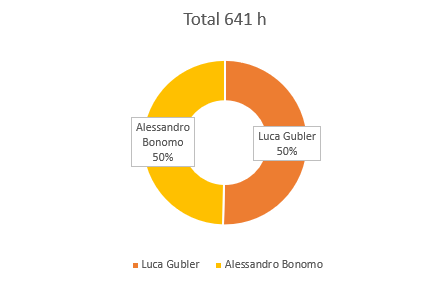
\includegraphics[width=0.8\textwidth, height=\textheight, keepaspectratio]{images/Zeitauswertung/Arbeitsaufwand_Personen.png}
		\caption{Zeitaufwand nach Mitgliedern}
		\label{time_per_student}
		\end{center}
\end{figure}

In den Abbildungen \ref{time_per_phase} und \ref{time_per_phase_and_person} ist der prozentuale Aufwand pro Phase, beziehungsweise der effektive Aufwand pro Projektmitglied und Phase, abgebildet.

	\begin{figure}[H]
\begin{center}

		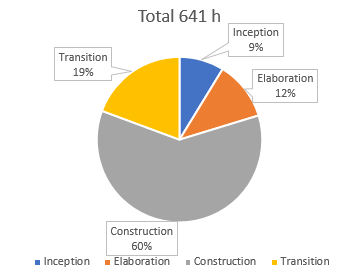
\includegraphics[width=0.8\textwidth, height=\textheight, keepaspectratio]{images/Zeitauswertung/Prozentualer_Aufwand_Phasen.png}
		\caption{Zeitaufwand nach Phasen}
		\label{time_per_phase}
	\end{center}		
\end{figure}

	\begin{figure}[H]
		\begin{center}
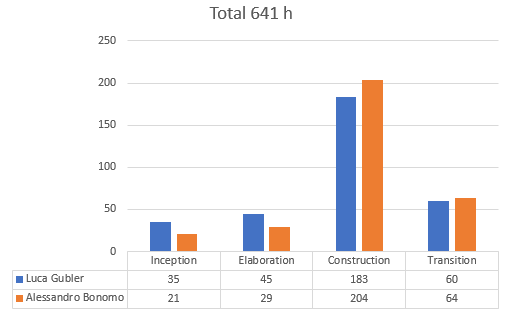
\includegraphics[width=0.8\textwidth, height=\textheight, keepaspectratio]{images/Zeitauswertung/Prozentualer_Aufwand_Phasen_Effektiv.png}
		\caption{Zeitaufwand nach Phasen und Person}
		\label{time_per_phase_and_person}
		\end{center}		
\end{figure}

Die Abbildung \ref{time_per_Week} zeigt, wie viel Zeit jedes Projektmitglied pro Woche in die Arbeit investiert hat. Durch Job und andere Module, entstanden gewisse Schwankungen über das Semester verteilt. Dennoch ist es beiden Projektmitgliedern gelungen, den geforderten Zeitaufwand von je 300 Studnen zu leisten.

	\begin{figure}[H]
				\begin{center}
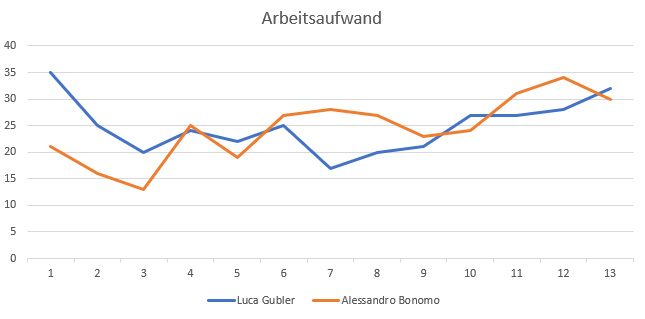
\includegraphics[width=0.8\textwidth, height=\textheight, keepaspectratio]{images/Zeitauswertung/Aufwand_Wochen.png}
		\caption{Zeitaufwand pro Woche}
		\label{time_per_Week}
		\end{center}		
\end{figure}


